\documentclass[12pt,a4paper]{scrartcl}
\usepackage[english,russian]{babel}
\usepackage{amsmath}
\usepackage{amsfonts}
\usepackage[utf8]{inputenc}
\usepackage{indentfirst}
\usepackage{misccorr}
\usepackage{graphicx}
\usepackage{commath}
\usepackage{calc}
\usepackage{mathrsfs}
\usepackage{csquotes}
\usepackage{caption}
\usepackage{listings}
\usepackage{xcolor}
\usepackage{hyperref}


\definecolor{codegreen}{rgb}{0,0.6,0}
\definecolor{codegray}{rgb}{0.5,0.5,0.5}
\definecolor{codered}{rgb}{0.9,0,0}
\definecolor{backcolour}{rgb}{0.95,0.95,0.92}
\definecolor{refcolor}{HTML}{00CC66}

\lstdefinestyle{mystyle}{
    backgroundcolor=\color{backcolour},   
    commentstyle=\color{codegreen},
    keywordstyle=\color{orange},
    numberstyle=\tiny\color{codegray},
    stringstyle=\color{codered},
    basicstyle=\ttfamily\footnotesize,
    breakatwhitespace=false,         
    breaklines=true,                 
    captionpos=b,                    
    keepspaces=true,                 
    numbers=left,                    
    numbersep=5pt,                  
    showspaces=false,                
    showstringspaces=false,
    showtabs=false,                  
    tabsize=2
}

\lstset{style=mystyle}

\hypersetup{pdfstartview=FitH, linkcolor=refcolor, urlcolor=refcolor, colorlinks=true}

\graphicspath{{images/}}

\begin{document}
\begin{flushright}
    Некрасов В. В., 225г.
\end{flushright}
\begin{center}
    \Large \textbf{Отчёт по задаче №13}\\
    <<Невидимая подпись изображения>>
\end{center}

\section{Задача} 
Программа должна загрузить графические изображения из файлов \texttt{InputFile1} и \texttt{InputFile2}, заменить в первом изображении все пикселы, не равные соответствующим пикселам второго изображения, на пикселы первого изображения с ближайшим значением и вывести полученный результат в файл \texttt{OutputFile} (с помощью данной процедуры можно создавать невидимую подпись изображения). Размер полученного изображения равен размеру первого изображения. 

\section{Создание изображений с подписью}
Создадим два изображения в формате BMP:
\begin{figure}[h]
    \begin{minipage}[h]{0.49\linewidth}
        \center{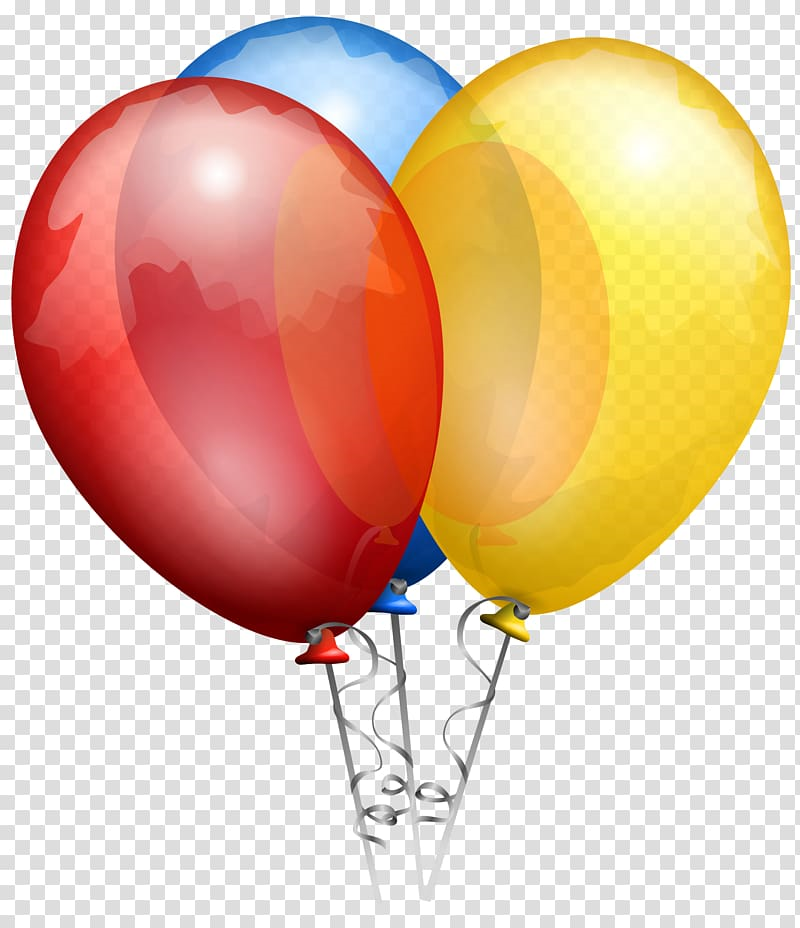
\includegraphics[scale=0.28, bb=5 10 800 928]{ball.png}  \\ ball.bmp}
    \end{minipage}
    \hfill
    \begin{minipage}[h]{0.49\linewidth}
        \center{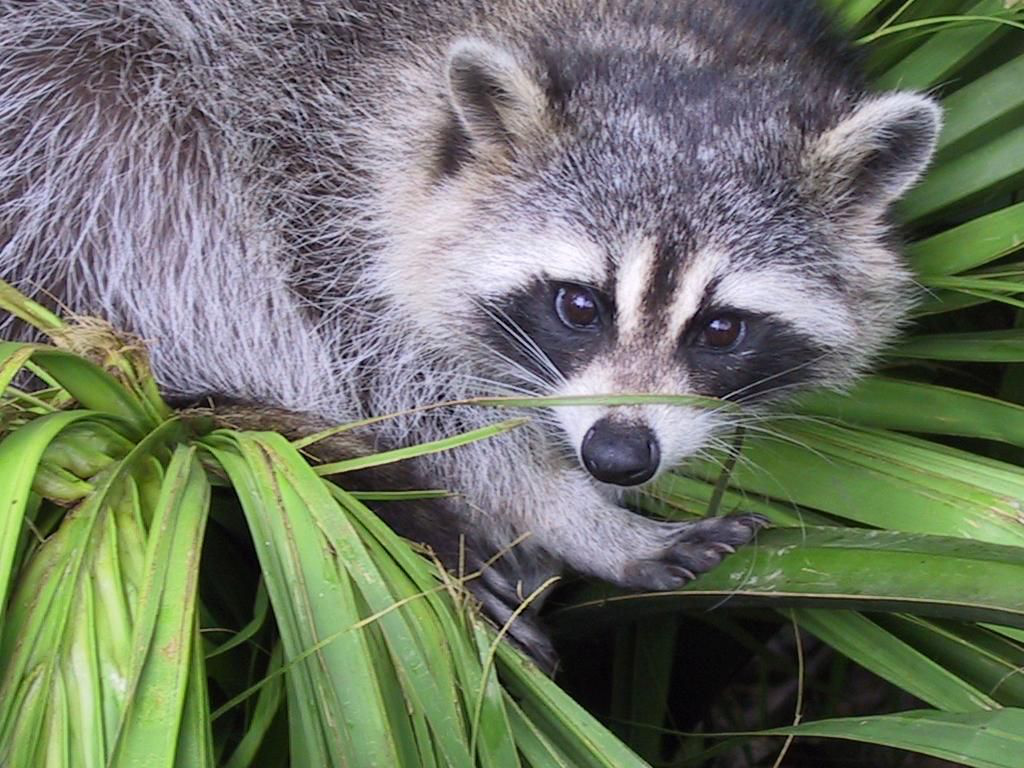
\includegraphics[scale=0.23, bb=5 10 1024 768]{face.png}  \\ face.bmp}
    \end{minipage}
    \caption{Исходные изображения.}
    \label{im:1}
\end{figure}

Кроме этого, с помощью программы GIMP подпишем созданные изображения  \hyperref[im:1]{рис. \ref*{im:1}}:
\begin{figure}[h]
    \begin{minipage}[h]{0.49\linewidth}
        \center{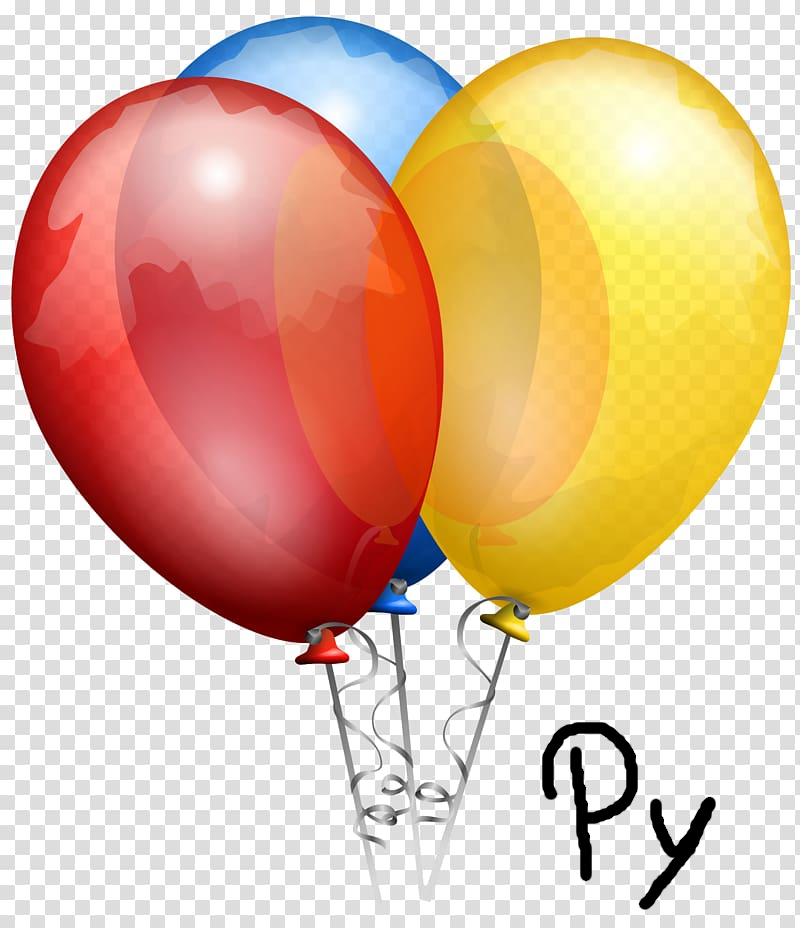
\includegraphics[scale=0.28, bb=5 10 800 928]{ball_sign.png}  \\ ball\_sign.bmp}
    \end{minipage}
    \hfill
    \begin{minipage}[h]{0.49\linewidth}
        \center{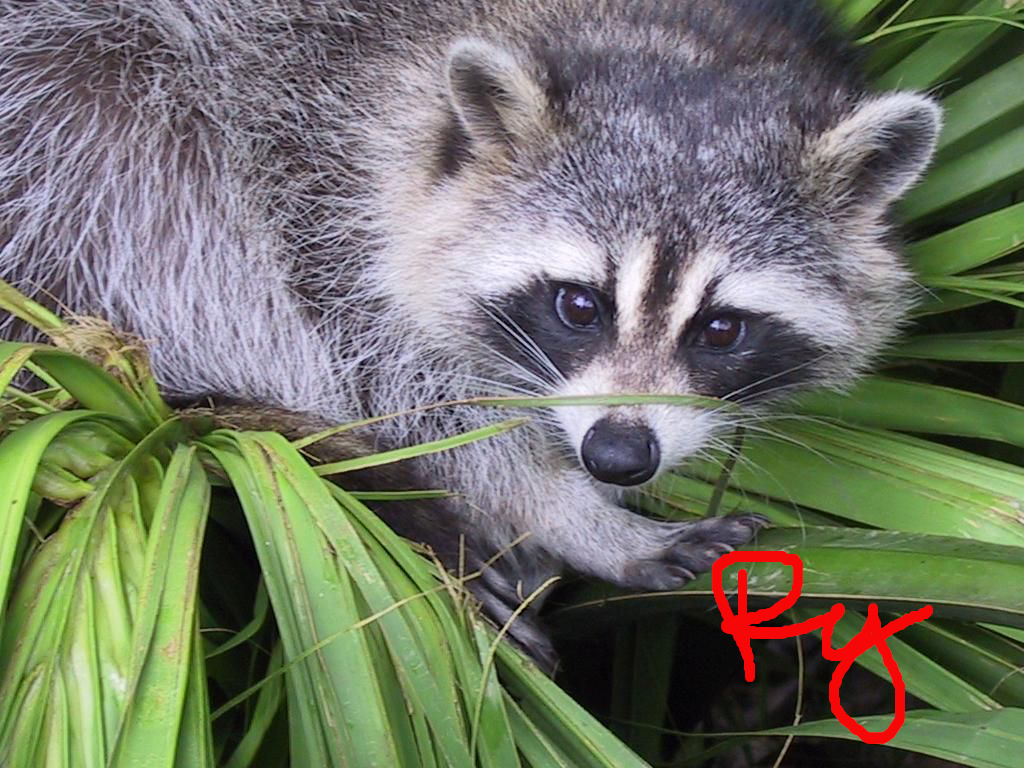
\includegraphics[scale=0.23, bb=5 10 1024 768]{face_sign.png}  \\ face\_sign.bmp}
    \end{minipage}
    \caption{Подписанные изображения.}
    \label{im:2}
\end{figure}
\newpage
\section{Программа, скрывающая подпись}
Напишем программу \texttt{make\_invisible\_sign.py}, создающую невидимую подпись.
Подключим необходимые библиотеки и загрузим изображения из файлов с учётом ошибок. Напечатаем ширину и высоту изображения:
\begin{lstlisting}[language=Python]
    from imageio import imread, imwrite
    import sys
    import numpy as np

    global im_sign, im_unsign, h, w #global for using in all functions
    if len(sys.argv) == 4: #if not enough args in command line
        im_unsign = imread(sys.argv[1]) #unsigned image
        im_sign = imread(sys.argv[2]) #signed image
        
    else:
        print("err")
        exit()
    h = len(im_sign)
    w = len(im_sign[0])
    print('width = ', w, 'height = ', h)
\end{lstlisting}

Сделаем функцию, возвращающую ближайший пиксел к заданной точке, но не совпадающий с ней. Для этого в окрестности заданной точки будем искать пиксел, расстояние (в смысле линейного пространства RGB) от которого до заданной точки будет минимальным. Если такой пиксел нашёлся, то его и будем считать ближайшим, а если такого нет (например, всё изображение одного цвета), то в качестве ближайшего пиксела выберем исходный с изменённой компонентой Blue на единицу. Минимальное расстояние задается из условия, что ближайшие цвета должны всё-таки отличаться не сильно (можно регулировать):
\begin{lstlisting}[language=Python]
def nearest(pix, pix_i, pix_j):
    nearest_pix = [0,0,0]
    min_dist = 100
    for i in range(5):
        for j in range(5):
            next_pix = im_unsign[pix_j + j][pix_i + i]
            if np.linalg.norm(next_pix - pix) < min_dist \
            and list(next_pix) != list(pix): 
            #list() is used to compare three RGB components 
                min_dist = np.linalg.norm(next_pix - pix)
                nearest_pix = next_pix 
                
    if list(nearest_pix) == [0,0,0]:
        nearest_pix = pix
        if nearest_pix[2] > 0:
            nearest_pix[2] -= 1
        else: 
            nearest_pix[2] += 1
    
return nearest_pix
\end{lstlisting}

Пройдёмся по всёму изображению. Если найдётся пиксел, который не совпадает в исходном и подписанном изображениях, то такой пиксел меняем на ближайший:
\begin{lstlisting}[language=Python]
for i in range(w):
    for j in range(h):
        if list(im_sign[j][i]) != list(im_unsign[j][i]): 
            im_sign[j][i] = nearest(im_unsign[j][i], i, j)

im_sign = imwrite(sys.argv[3], im_sign)    
print("Unvisible sign is done!")
\end{lstlisting}    
Вызываем программу из командной строки с параметрами \texttt{InputFile1} \texttt{InputFile2} \texttt{OutputFile}:
\begin{lstlisting}
python make_invisible_sign.py face.bmp face_sign.bmp out_face.bmp
python make_invisible_sign.py ball.bmp ball_sign.bmp out_ball.bmp
\end{lstlisting}
Получим изображения c невидимой подписью: \hyperref[im:3]{рис. \ref*{im:3}}.
\begin{figure}[h]
    \begin{minipage}[h]{0.49\linewidth}
        \center{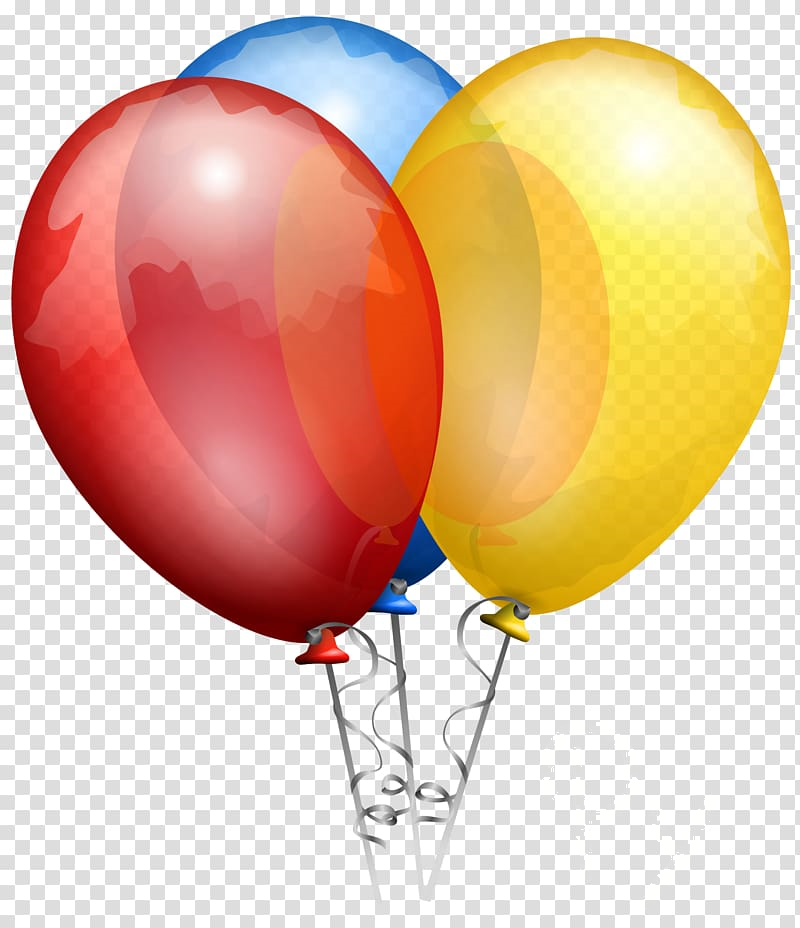
\includegraphics[scale=0.28, bb=5 10 800 928]{out_ball.png}  \\ out\_ball.bmp}
    \end{minipage}
    \hfill
    \begin{minipage}[h]{0.49\linewidth}
        \center{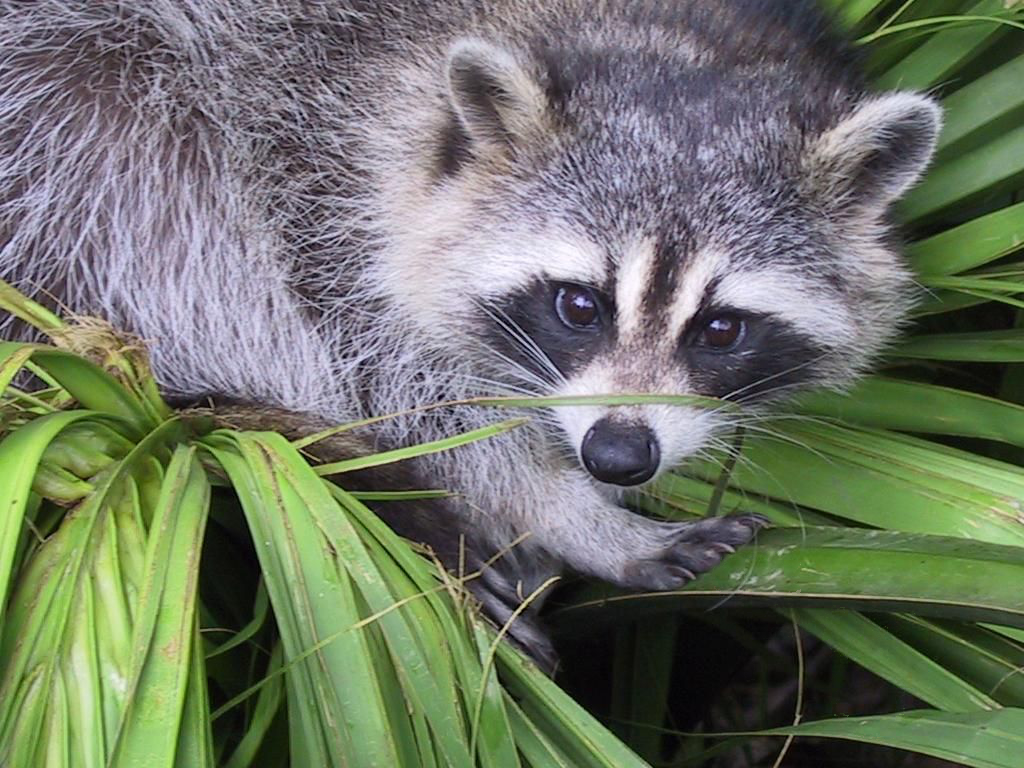
\includegraphics[scale=0.23, bb=5 10 1024 768]{out_face.png}  \\ out\_face.bmp}
    \end{minipage}
    \caption{Изображения с невидимой подписью.}
    \label{im:3}
\end{figure}

\section{Программа, проявляющая невидимую подпись}
Как можно видеть на \hyperref[im:3]{рис. \ref*{im:3}}, невидимую подпись различить глазом практически невозможно.
Поэтому создадим \hyperref[issign]{программу} \texttt{is\_signed.py}, которая по данному и исходному изображениям выясняет, было ли подписано данное изображение, в том числе, невидимой подписью, и проявляет эту подпись чёрным цветом.
\newpage
\vspace*{-0.5cm}
Программа \texttt{is\_signed.py}: 
\lstinputlisting[language=Python, label=issign]{is_signed.py}
Эту программу можно вызвать из командной строки следующим образом:
\begin{lstlisting}
python3 is_signed.py face.bmp face.bmp out_face_sign.bmp
python3 is_signed.py ball.bmp out_ball.bmp out_ball_sign.bmp
\end{lstlisting}
Её работу демонстрируют полученные изображения:
\begin{figure}[h]
    \begin{minipage}[h]{0.49\linewidth}
        \center{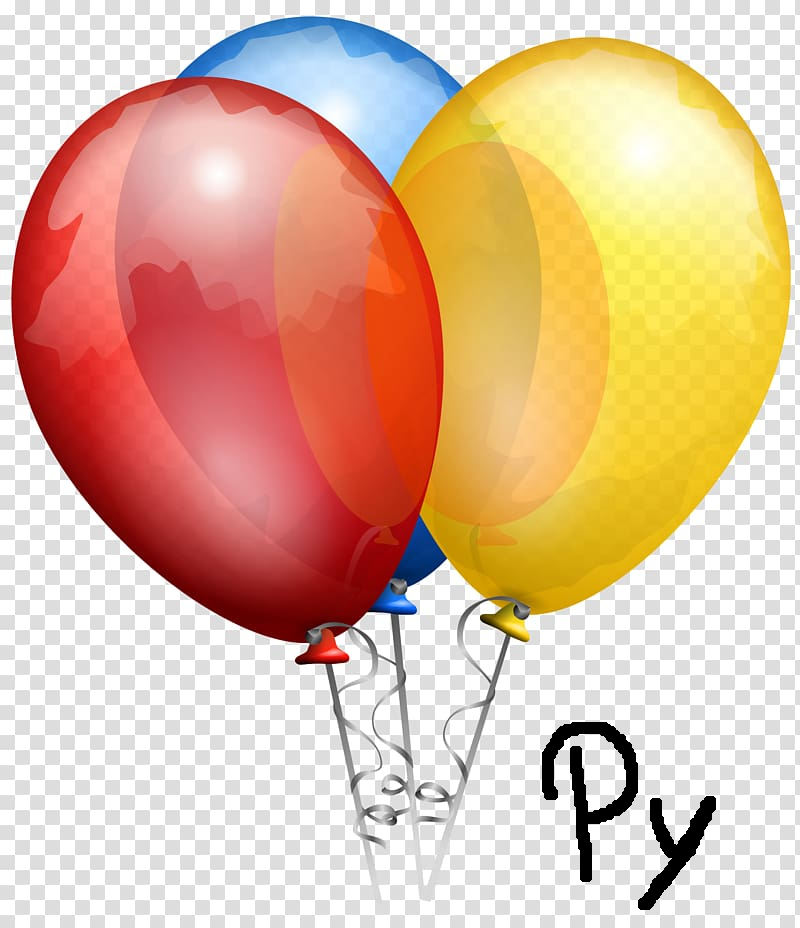
\includegraphics[scale=0.28, bb=5 10 800 928]{out_ball_sign.png}  \\ out\_ball\_sign.bmp}
    \end{minipage}
    \hfill
    \begin{minipage}[h]{0.49\linewidth}
        \center{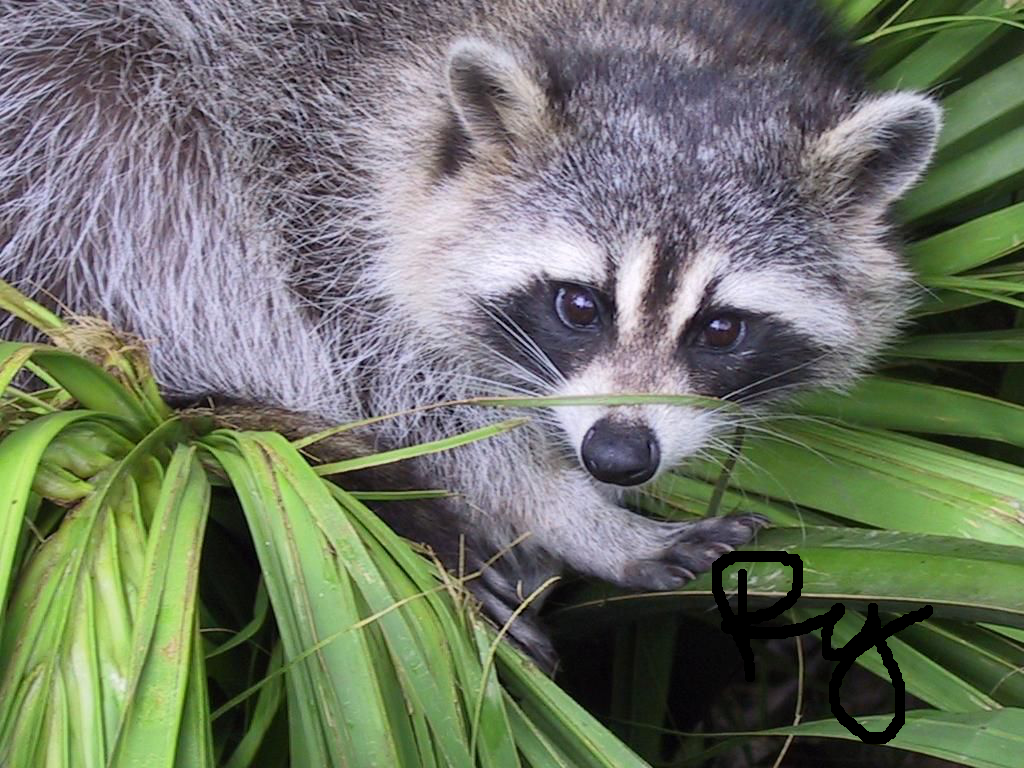
\includegraphics[scale=0.23, bb=5 10 1024 768]{out_face_sign.png}  \\ out\_face\_sign.bmp}
    \end{minipage}
    \caption{Изображения с проявленной невидимой подписью.}
    \label{im:4}
\end{figure}

\section{Оценка результатов}
Итак, программа \texttt{make\_invisible\_sign.py} получает на вход изображение с подписью и без подписи и создает по ним изображение с невидимой подписью. Программа \texttt{is\_signed.py} позволяет выяснить, было ли изображение подписано, и проявить подпись, если она была. В случае однородного по цветам изображения невидимая подпись немного видна, но если же подпись поставлена на изображении, где много различных близких цветов (например, фотография), то тогда невидимую подпись заметить глазом невозможно.

Файлы программ и картинки можно найти по ссылке: 

\href{https://github.com/Harrix/Math-Harrix-Library}{https://github.com/Harrix/Math-Harrix-Library}
\end{document}
